%% LyX 2.5.0~devel created this file.  For more info, see https://www.lyx.org/.
%% Do not edit unless you really know what you are doing.
\documentclass[english]{article}
\usepackage[T1]{fontenc}
\usepackage{array}
\usepackage{booktabs}
\usepackage{multirow}
\usepackage{amssymb}
\usepackage{graphicx}
\usepackage{tablefootnote}
\usepackage{setspace}
\usepackage{url}

\makeatletter

%%%%%%%%%%%%%%%%%%%%%%%%%%%%%% LyX specific LaTeX commands.
%% Because html converters don't know tabularnewline
\providecommand{\tabularnewline}{\\}
%% A simple dot to overcome graphicx limitations
\newcommand{\lyxdot}{.}


%%%%%%%%%%%%%%%%%%%%%%%%%%%%%% User specified LaTeX commands.
\usepackage {a4wide}
\usepackage{times}

\ifdefined\showcaptionsetup
 % Caption package is used. Advise subfig not to load it again.
 \PassOptionsToPackage{caption=false}{subfig}
\fi
\usepackage{subfig}
\makeatother

\usepackage{babel}
\begin{document}
\title{Exploring Smartphone-Based Edge Computing \\ for AI Inference using
Real Testbeds}
\maketitle
\begin{abstract}
Gradually, AI is becoming ubiquitous at the network edge. The wide
availability of pre-trained models and AI execution frameworks contribute
to such ubiquity. Particularly, deep learning (DL) models such as
convolutional neural networks (CNN) are extensively used in computer
vision (CV) for performing object recognition and image classification
tasks. Solutions in various domains ranging from security surveillance
to e-health exploit computer vision tasks. In many cases, such solutions
must deliver realtime inferences; some progress has been made in this
respect. Some approaches show a strong dependency on Cloud resources
as complements to the computing power that resource limited edge nodes
can offer. Other solutions distribute workload horizontally, i.e.,
by harnessing the power of several edge nodes within the same LAN
or WLAN. Many of these efforts experiment with real settings comprising
SBC-like (Single Board Computers) edge nodes only such as NVidia Jetson
Nano and Raspberry Pi; few of these consider nomadic hardware such
as smartphones as edge nodes. Given the ubiquity of smartphones worldwide
and the unlimited scenarios where clusters of these nodes can be exploited
for providing substantial computing power, in this work, we shed some
light in answering the following question: Is smartphone-based edge
computing a competitive resource provider for realtime AI inferences?
We evaluate the potential of smartphone clusters for making realtime
inferences associated to CV tasks based on intuitive image/video partitioning
schemes. In our experiments we use three pre-trained DL models that
present different computing requirements and eight heterogeneous edge
nodes including five low/mid-end smartphones and three SBCs. We compared
the performance achieved using workloads from three image stream processing
scenarios with different characteristics. Experiments were run with
the help of a tool set designed for reproducing battery-driven edge
computing tests. We compared latency and energy efficiency achieved
by using either several smartphone clusters testbeds or SBCs only.
Additionally, for battery-driven settings, we include metrics to measure
how workload execution impact smartphone battery levels. As per the
computing capability shown in our experiments, we conclude that edge
computing based on smartphone clusters can help in providing valuable
computing resources to enable the expansion of AI in application scenarios
requiring realtime responses.
\end{abstract}

\section{Introduction}

The application of deep learning (DL) to perform on-site tasks is
rapidly expanding. In the healthcare domain, DL is used for predicting,
detecting, diagnosing, and prognosing different diseases~\cite{NguyenDeepEnsemble2021,MahajanEnsemble2023}.
In food production, particularly, animal farming~\cite{bao2022artificial}
these tasks include animal behavior recognition, growth evaluation,
and individual identification. In the smart city domain~\cite{ullah2020applications,javed2023survey},
tasks include intelligent transportation, waste management, crime
prediction, public infrastructure and green spaces maintenance. Many
of these tasks involve object classification and recognition using
images as input. The application of CNNs (Convolutional Neural Networks)
has become popular to perform these tasks due to the training procedure
requiring minimal human intervention compared to other machine learning
techniques. However, training a deep neural network model requires
big datasets and powerful hardware. Nowadays, data gathering leveraged
by mobile and IoT devices, and computing power offered by cloud computing
platforms, greatly speeds up such training process compared to a couple
of decades ago. Cloud computing is considered not only in the training
phase of DL models but also for making inferences. It implies that
a trained model deployed in a remote computing infrastructure is evaluated
with locally-generated input data, and produces output results that
must be transferred back traversing long-latency Internet uplinks
and downlinks. This latency has been been identified a limitation
for time-sensitive applications. To overcome this issue and others
such as unavailability of the Internet connection, network overloading
and privacy protection, edge-based architectures have been proposed~\cite{yousefpour2019all,ray2019minimizing}.

There are differences highlighted in the literature when referring
to edge-based architectures~\cite{yousefpour2019all}, some of these
being simply terminological, and some others describing substantial
differences in the way their constituent components are defined and
interoperate with components from other computing layers~\cite{vsojat2020rainbow}.
Points in common, however, are minimizing data transportation and
bringing computing resources close to where computing needs and data
originate. Heterogeneity and energy constraints are common features
of computing infrastructures operating in cyber-physical and IoT systems.
For these reasons, cooperation is a key concept of \emph{Dew Computing}~\cite{gusev2018formal},
which is among these edge-based architectures and endows low processing
power and consumer devices with the role of main computing resource
providers.

In this work, we focus on evaluating collaboration among consumer
devices to perform cloud-agnostic computing services for realtime
execution of computer vision tasks using DL. The contributions of
this work can be summarized as follows:
\begin{itemize}
\item We applied an intuitive data partition scheme to create and distribute
CV tasks among clusters of smartphones for performing real-time inferences
over data streams workloads with different characteristics. 
\item We evaluated and compared using real testbeds the performance and
energy consumption of smartphone clusters against typical edge nodes
including SBCs, explaining some implications of the results obtained.
\item The evaluated scenarios serve as a guide and example on how to use
previously published tools especially designed to facilitate the experimenation
with real testbeds comprising smartphone clusters.
\end{itemize}
This work is organized as follows. Section~\ref{sec:Related-works}
presents and classifies recent efforts backed by real testbeds results
to speed up inferences at the edge using different approaches for
distributed execution. Section~\ref{sec:System-model-=000026-assumptions}
describes the mobile distributed computing model and infrastructure-related
architectural assumptions we made in our exploration tests, as well
as details concerning DL models used and data stream workloads. In
Section~\ref{sec:Empirical-evaluation} we explain details about
node setups and metrics, results obtained in our empirical evaluation
and a discussion. Lastly, Section~\ref{sec:Conclusions-and-future}
presents the conclusions and future research directions.

\section{Related Works\protect\label{sec:Related-works}}

In this section we analyze different relevant works in line with the
broad concept of \emph{distributed inference}, which is present in
recent research related to AI at the network edge, and we define and
explore in the rest of the Section. In the context of AI, an inference
means asking a model to compute a result based on input data (e.g.,
given an image, list the objects detected). All mentioned works include
experimentation with real testbeds.
\begin{table}
\begin{centering}
\begin{tabular}{|c|c|}
\hline 
Distributed inference type & Associated works\tabularnewline
\hline 
\hline 
Vertical & \cite{kang2017neurosurgeon,huang2020deepadapter,huang2020lightweight,eshratifar2019jointdnn,teerapittayanon2017distributed}\tabularnewline
\hline 
Horizontal & \cite{guo2023automated,huang2022toward,taufique2024adaptive,zhao2018deepthings,huang2021enabling}\tabularnewline
\hline 
\end{tabular}
\par\end{centering}
\caption{Approaches for distributed inference}

\end{table}

When computing infrastructures of at least two nodes perform inference
tasks, it is said that distributed inference is applied. The scheme
under which such a distribution is given can be vertical~\cite{kang2017neurosurgeon,eshratifar2019jointdnn,teerapittayanon2017distributed}
or horizontal~\cite{guo2023automated,huang2022toward,taufique2024adaptive,zhao2018deepthings,huang2021enabling}.
Under the vertical scheme, collaborating nodes typically belong to
different computing layers of the edge architecture. These layers
are organized in a hierarchical structure where nodes in a layer render
services to those in the layer below using services provided by nodes
in the layer above. Nodes at the base of such hierarchy commonly have
much less powerful computing capabilities and use the services of
layers above to complete computationally intensive tasks. On the other
side, nodes at the top layer present more powerful computing capabilities,
like Fog or Cloud resources. However, reaching such nodes incur in
long-latency communication when transferring task input/output data.
For this reason, its usage should be carefully analyzed especially
for applications with delay-sensitive time constrains. A classical
example of this type of collaboration is given when a resource-limited
user device leverages the services of an Edge server or Edge layer
to partially o completely compute the result of inference tasks. Since
the Edge layer can render computing services to a variable number
of users in a locality, depending on the burden at the time of receiving
tasks, the Edge layer can have enough resources to complete or partially
perform a task. In the later case, the Edge layer would eventually
leverage the services of a remote cloud datacenter to fullfill the
request while meeting potential task deadlines. Like in~\cite{eshratifar2019jointdnn,kang2017neurosurgeon},
offloading decisions are evaluated considering communication throughput
between computing layers. Besides, a task requiring the execution
of a DL model is split into several parts. In this splitting process
authors propose to consider insights of data anatomy and computing
requirements of layers characterizing different DL models. Partitions
of model's graph are dynamically assigned and executed between a device
and remote servers. Other works adopting this distribution scheme
are the ones by \cite{huang2020lightweight,huang2020deepadapter,teerapittayanon2017distributed}.
Several works evidence that vertical collaboration is feasible to
allow resource-limited devices to execute compute-intensive tasks,
such as CV tasks using large DL models. However, a major drawback
relates to the long-latency communication dependency when offloading
tasks to upper resource layers that provide the required computing
capability to complete the tasks.

\begin{singlespace}
Another inference distribution scheme is when nodes within the same
layer collaborate in the execution of compute intensive tasks. This
scheme is known as horizontal collaboration. A key difference with
vertical collaboration is that participating nodes and data rarely
occurs outside the scope of a LAN or WLAN. Even though this form of
collaboration governs the internal communication of nodes within the
same layer, in this paper, we put special focus on the horizontal
communication of resource-constrained nodes including edge and user
device nodes. In the literature, we have identified several works
proposing distributed inference under this form of collaboration~\cite{guo2023automated,huang2022toward,taufique2024adaptive,zhao2018deepthings,huang2021enabling}
that we further analyzed taking into account several dimensions. Namely,
the type of parallelism proposed, i.e., whether it is by intervening
the anatomy of a DL model, partitioning the data input or adopting
a hybrid approach by combining the previous techniques. Other dimension
of analysis relates to the methodology used to evaluate the proposal.
We selected works whose methodology involves setting up real testbeds
and describe the hardware used and the way resource heterogeneity
is present in the experiments. Moreover, providing that QoS is a concept
that relates to adapting to dynamic changes in the workload and/or
available resources, we indicate the support of these works in this
respect. Finally, we contextualize the strategy of each work for resource
management mentioning the main motivation behind the proposal.

{\footnotesize{}
\begin{table}
{\footnotesize{}%
\begin{tabular}{>{\centering}p{1.5cm}>{\raggedright}p{2cm}>{\raggedright}p{2cm}>{\centering}p{3cm}>{\centering}p{3cm}>{\centering}p{1cm}}
\toprule 
\multirow{2}{1.5cm}{{\footnotesize Parallelism type}} & \multicolumn{2}{c}{{\footnotesize Experiments}} & \multirow{2}{3cm}{{\footnotesize Online adaptive QoS support?}} & \multirow{2}{3cm}{{\footnotesize Main motivation}} & \multirow{2}{1cm}{{\footnotesize Work}}\tabularnewline
\cmidrule{2-3}
 & {\footnotesize Resource heterogeneity type} & {\footnotesize Type} &  &  & \tabularnewline
\midrule
\midrule 
\multirow{2}{1.5cm}{{\footnotesize Model Partitioning}} & {\footnotesize Homogeneous nodes; varying resource type and quantity
--CPU Cores and GPU--} & {\footnotesize Real hardware: LAN with up to eight edge devices (Nvidia
Jetson Xavier NX)} & {\footnotesize No (once generated and deployed, mappings between sub-model
and edge nodes are fixed at runtime)} & {\footnotesize Automate large CNN model partitioning, deployment and
execution on multiple resource-constrained edge devices} & {\footnotesize\cite{guo2023automated}}\tabularnewline
\cmidrule{2-6}
 & {\footnotesize Homogeneus nodes; varying CPU usage and network bandwidth} & {\footnotesize Real Hardware: LAN with three IoT devices (Raspberry
Pi 4)} & {\footnotesize Yes (uses a Deep Reinforcement Learning-based adaptive
allocator and a fault tolerant mechanism implemented using a message
queue)} & {\footnotesize Accelerate performance with an intra-layer parallelism
instead of layers sequential execution as in traditional hierarchical
inference} & {\footnotesize\cite{huang2022toward}}\tabularnewline
\midrule 
\multirow{2}{1.5cm}{{\footnotesize Data partitioning}} & {\footnotesize Heterogeneous nodes (IoT devices)} & {\footnotesize Real Hardware: LAN with four IoT devices (2x Odroid
XU4, Jetson Nano, Rapsberry Pi 4)} & {\footnotesize Yes (accuracy-performance-heterogeneity tradeoffs exploitation)} & {\footnotesize Exploit the concept of approximate computing to ensure
performance and accuracy constraints considering heterogeneity of
the edge cluster and nodes availability} & {\footnotesize\cite{taufique2024adaptive}}\tabularnewline
\cmidrule{2-6}
 & {\footnotesize Heterogeneous nodes (Smartphones}{\footnotesize\par}

{\footnotesize and IoT devices)} & {\footnotesize Real Hardware: WLAN of different smartphones clusters
size. IoT devices operating in isolated mode} & {\footnotesize Yes (pull-based scheme using a shared workload queue)} & {\footnotesize Compare inference delivery capabilities and energy efficiency
of IoT devices versus clusters of smartphones} & {\footnotesize This work}\tabularnewline
\midrule 
\multirow{2}{1.5cm}{{\footnotesize Hybrid}} & {\footnotesize Homogeneous nodes; varying number of available devices} & {\footnotesize Real Hardware: WLAN with up to six IoT devices (Raspberry
Pi 3)} & {\footnotesize Yes (work stealing)} & {\footnotesize Allow large DL models to execute in resource limited
devices achieving low memory footprint and execution latency} & {\footnotesize\cite{zhao2018deepthings}}\tabularnewline
\cmidrule{2-6}
 & {\footnotesize Heterogeneous nodes (smartphones)} & {\footnotesize ion: with data profiled from hardware running real workloads}\\
{\footnotesize Real Hardware: some real experiments} & {\footnotesize Yes (uses Deep Reinforcement Learning)} & {\footnotesize Reduce Mobile Edge Computing server's computing pressure} & {\footnotesize\cite{huang2021enabling}}\tabularnewline
\bottomrule
\end{tabular}}{\footnotesize\par}

{\footnotesize\caption{Approaches for horizontal distributed inference at the Edge}
}{\footnotesize\par}
\end{table}
}{\footnotesize\par}

Works can be also classified according to how workload execution is
parallelized. We found three approaches of parallelism named model
partitioning, data partitioning, and hybrid. Within the former group,
layers composing a DL model are deployed into different devices so
that outputs computed by a device are the inputs for another one.
With this type of parallelism, all participating devices are involved
in computing inferences for all portions of the input. By contrast,
when using data partitioning paralellism, edge nodes run the whole
model over portions of the input. A third type, which we call hybrid,
parallelizes workload by combining the data and model partitioning
schemes. In all cases, results for the whole input are obtained by
joining partial results calculated by all participating devices.
\end{singlespace}

When making several devices to participate in inferences, two questions
related to devices emerge: Does the approach consider executing inferences
on heterogeneous devices? If so, what does the approach do to deal
with the performance differences from executing the same workload
on devices with different computing capabilities in order to assure
certain QoS levels?

In~\cite{guo2023automated}, authors propose AutoDiCE, a tool for
partitioning, deploying, and distributedly executing a large CNN model
on multiple resource-constrained edge devices. The platform specification
and mapping specification allow practitioners to indicate which submodel
runs on which edge devices. Communication between sub-models and resources
usage is implemented via the well-known parallel programming standards
MPI and OpenMP. Although the tool was designed to support horizontally
and vertically distributed inferences, it was tested using the former
scheme, using an infrastructure comprising homogeneous edge nodes
communicated via a gigabit Ethernet switches. DeColla~\cite{huang2022toward}
utilizes Deep Reinforcement Learning (DRL)-based adaptive allocation
for horizontal collaborative inference. All DL layers are present
in all collaborating IoT devices. Neurons calculation of each layer
occurs in parallel, coordinated via a message queue and orchestrated
by DeColla engine that operates in a requester IoT device. Number
of IoT devices, available computing resources, and the network state
are evaluated online upon each neuron assignment.

In~\cite{taufique2024adaptive} the most appropriate version among
different pruned models is selected online via an adaptive workload
distribution to meet the required application specific accuracy and
performance level. Such dynamic selection is performed using a base
knowledge of accuracy-performance tradeoffs profiled from heterogeneous
edge nodes, together with a runtime monitoring system for resource
management. In~\cite{zhao2018deepthings} the DeepThings framework
for executing large CNN models in resource-constrained devices is
proposed. The framework adopts a hybrid parallelization approach due
to it combines model and data partitioning schemes. On one side, as
an offline step the framework fused convolutional and pooling layers
to create independent and distributable execution units, which leads
to reduced memory footprint and allow resource limited devices to
contribute with the computation of partial results that are combined
to produce the final result of an inference task. Besides, workload
represented by a single frame is divided into overlapping and distributable
regions that are computed collaboratively by a group of edge devices.
With this scheme, inference capabilities differences of participating
devices are handled with two strategies. One of these is static and
represented by the fact that memory requirements of fused layers executed
by a device adapts to its available memory resources. The other strategy
is that data regions are dynamically distributed according to devices
computing capabilities by following a work stealing scheme. Another
work adopting hybrid paralelization is eDDNN~\cite{huang2021enabling},
which leverages cross-platform Web technologies and WebRTC protocol
to allow for distributed inference among end devices. The collaboration
is mediated by an edge server that keeps track of nodes and tasks
status information. Tasks, determined by images input size, and the
DL model to be used, are divided into sub-images and sub-models by
a decision maker component that coordinates different pieces execution
among end devices using a shared dependency table and realtime nodes
information. Edge data duplication is present at the step of dividing
an image into sub-images. When distributing a convolutional operation
by dividing the input and the model, duplication is required for ensuring
results correctness.

In the discussed works, horizontal distributed inference considering
the collaboration of battery-operated end-user devices, such as smartphones,
combined with data partitioning schemes are scarce, meaning that the
benefits and limitations of performing realtime CV tasks --and possibly
other AI tasks as well-- are yet unknown. Our work sheds light on
providing empirical evidence for quantifying the computing power of
smartphone clusters. Existing approaches exploiting data partitioning
schemes add redundant data to the original input for performing distributed
inference. We propose a simple yet effective data partitioning scheme
for performing realtime CV tasks, which is evaluated under varying
settings of real smartphones cooperating in WLAN clusters. Since performance
may vary according to how workload is distributed, we provide insights
on the performance achieved and energy-related measurements using
different state-of-the-art online heuristics and smartphone clusters.
Moreover, performance comparisons of different <smartphone clusters,
load balancing heuristics> combinations were compared against the
performance achieved by different edge nodes commonly used in IoT
applications. All experiments performed in this work demonstrate the
viability of constructing a platform for in-vivo experiments whose
main components has been previously published, validated and made
publicly available for use~\cite{mateos2022LiveDewStream,yannibelli2024bagess,toloza2022motrol}.

\section{System Model and Assumptions\protect\label{sec:System-model-=000026-assumptions}}

We envision a system that opportunistically scavenges computing cycles
of nomadic hardware, such as smartphones, to complement -- or eventually
replace -- the computing cycles delivered by low power edge nodes.
Particularly, we shed light on the computing capability of different
smartphone clusters and load balancing heuristics for processing streams
at the Edge. In this work, we consider streams of images analyzed
using CV tasks in realtime or near realtime by harnessing deep neural
networks. Definition of appropriate incentives for smartphone users
-- tasks executors --, privacy preservation and security mechanisms
for tasks submitters as for tasks executors, are outside the scope
of the current work~\cite{li2019online,hou2020data,xu2019edge}.

We assume a master-worker architecture operating within the scope
of WLAN, with a master node officiating as tasks submitter and worker
nodes contributing with computing resources, i.e., playing the role
of tasks executors. A master node is assigned the roles of data concentrator
and tasks coordinator. Playing the first role implies that the node
exposes end points for receiving raw data and preprocessed data. On
one side, raw data transferred to a master node is captured by devices
with sensing capabilities, e.g., RGB, IR or depth images taken with
different camera devices. On the other side, pre-processed data is
obtained by applying a series of computational operations to decode,
synthesize and/or represent raw data in a format that can be more
efficiently stored, retrieved or analyzed. Moreover, playing the role
of tasks coordinator means that the node runs logic to decide how
to distribute the load involved in preprocessing raw data by available
worker nodes to meet the expected QoS. Finally, worker nodes opportunistically
connected to the WLAN register through a master node service to contribute
with computing resources and wait for tasks assigned by the master
node. As tasks completion occurs at the worker nodes, results are
sent back to the master node.

\begin{figure}
\centering{}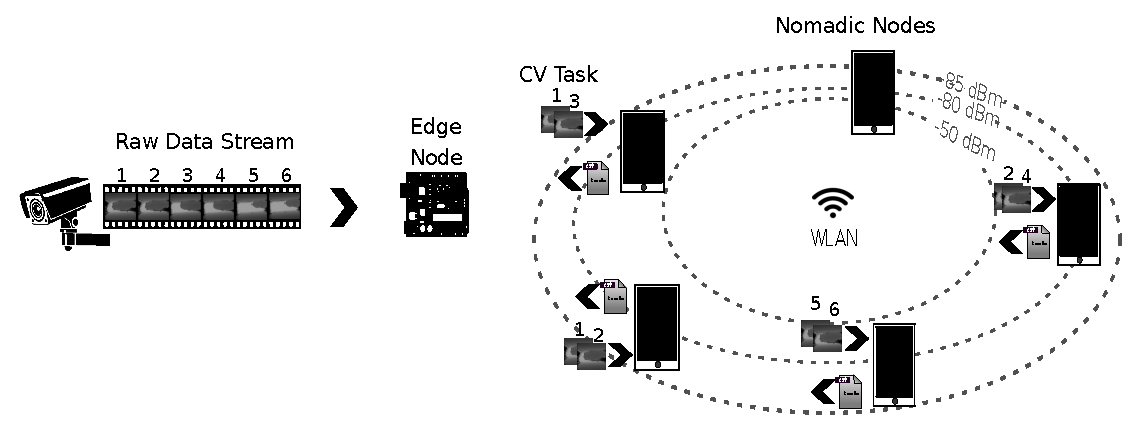
\includegraphics[scale=0.7]{figures/proxy-based_mdc}\caption{Main nodes schematic overview}
\end{figure}

With this architecture, we aim at measuring the feasibility of using
different smartphones groups cooperating under the same WLAN for performing
CV tasks, and compare the performance achieved with that of SBC-like
edge nodes commonly used for servicing IoT and edge applications.

\subsection{Empirical Evaluation\protect\label{sec:Empirical-evaluation}}

To conduct this study we employed different hardware as edge nodes,
whose characteristics are shown in Table~\ref{tab:Edge-nodes-features}.

\begin{table}
\begin{centering}
\begin{tabular*}{1\textwidth}{@{\extracolsep{\fill}}l>{\raggedright}p{0.12\columnwidth}>{\raggedright}p{0.05\columnwidth}>{\raggedright}p{0.2\columnwidth}>{\raggedright}p{0.1\columnwidth}>{\raggedright}p{0.1\columnwidth}>{\raggedright}p{0.07\columnwidth}>{\raggedright}p{0.07\columnwidth}}
\toprule 
\multicolumn{1}{>{\raggedright}p{0.03\columnwidth}}{{\scriptsize Edge Node Type}} & {\scriptsize Edge Node Name} & {\scriptsize Short name} & {\scriptsize Processor} & {\scriptsize RAM} & {\scriptsize Conectivity} & {\scriptsize Battery Capacity (mAh)} & {\scriptsize Avg. Price (USD)}\tabularnewline
\midrule
\midrule 
\multirow{3}{*}{{\scriptsize SBC}} & {\scriptsize Raspberry Pi 4} & {\scriptsize RPi4} & {\scriptsize Quad-core 1.5 GHz ARM Cortex-A72} & {\scriptsize 4 GB} & {\scriptsize Wi-Fi 802.11 ac} & {\scriptsize N/A} & {\scriptsize 55}\tabularnewline
\cmidrule{2-8}
 & {\scriptsize Nvidia Jetson Nano} & {\scriptsize NvJN} & {\scriptsize Quad-core ARM Cortex-A57 MPCore} & {\scriptsize 4 GB} & {\scriptsize Gigabit Ethernet, M.2 Key E} & {\scriptsize N/A} & {\scriptsize 99}\tabularnewline
\cmidrule{2-8}
 & {\scriptsize Gigabyte Brix GB-BRi5H-8250} & {\scriptsize GBx} & {\scriptsize Quad core i5-8250U} & {\scriptsize 8 GB} & {\scriptsize Wi-Fi 802.11 ac} & {\scriptsize N/A} & {\scriptsize 500}\tabularnewline
\midrule 
\multirow{5}{*}{{\scriptsize Smartphone}} & {\scriptsize Samsung A02} & {\scriptsize SamA02} & {\scriptsize Quad-core 1.5 GHz Cortex-A53} & {\scriptsize 2 GB} & {\scriptsize Wi-Fi 802.11 b/g/n} & {\scriptsize 4900} & {\scriptsize 116}\tabularnewline
\cmidrule{2-8}
 & {\scriptsize Motorola Moto G6} & {\scriptsize MotG6} & {\scriptsize Octa-core 1.8 GHz Cortex-A53} & {\scriptsize 3 GB} & {\scriptsize Wi-Fi 802.11 a/b/g/n} & {\scriptsize 3000} & {\scriptsize 160}\tabularnewline
\cmidrule{2-8}
 & {\scriptsize Samsung A30} & {\scriptsize SamA30} & {\scriptsize Octa-core (2x1.8 GHz Cortex-A73 \& 6x1.6 GHz Cortex-A53)} & {\scriptsize 3 GB} & {\scriptsize Wi-Fi 802.11 a/b/g/n/ac} & {\scriptsize 3900} & {\scriptsize 170}\tabularnewline
\cmidrule{2-8}
 & {\scriptsize Xiaomi Redmi Note 7} & {\scriptsize XRN7} & {\scriptsize Octa-core (4x2.2 GHz Kryo 260 Gold \& 4x1.8 GHz Kryo 260
Silver)} & {\scriptsize 4 GB} & {\scriptsize Wi-Fi 802.11 a/b/g/n/ac} & {\scriptsize 4000} & {\scriptsize 200}\tabularnewline
\cmidrule{2-8}
 & {\scriptsize Motorola Moto G9 Play} & {\scriptsize MotG9} & {\scriptsize Octa-core (4x2.0 GHz Kryo 260 Gold \& 4x1.8 GHz Kryo 260
Silver)} & {\scriptsize 4 GB} & {\scriptsize Wi-Fi 802.11 a/b/g/n/ac} & {\scriptsize 5000} & {\scriptsize 200}\tabularnewline
\bottomrule
\end{tabular*}
\par\end{centering}
\caption{Edge computing nodes: hardware features\protect\label{tab:Edge-nodes-features}}
\end{table}
 All nodes have multicore processors and all nodes but the Nvidia
Jetson Nano have 802.11 WiFi radio, with a theoretically bandwidth
capacity between hundreds of Mbps (norm n) to a few Gbps (norm ac).
In fact, SBC nodes WiFi was not used because, in our experiments,
these nodes play all the roles -- tasks submitter, tasks coordinator
and tasks executor -- simultaneously and no data transfers were involved.
Edge nodes main memory ranges from 2 to 8 GB. In our setups, SBC operate
plugged to the electricity power grid, while smartphones operate using
their battery as main power source. Additionally we included an estimated
per unit acquisition cost in USD. When searching for cost-effective
configurations, the cost can be used as a deciding factor in situations
where several nodes combinations achieved the desired performance.

Section~\ref{subsec:DNN-models-benchmarking} elaborates on the deep
learning models characteristics considered in the experiments. In
section~\ref{sec:workload-characterization} we describe three study
cases belonging to different application domains, how image streams
are produced, and task characteristics. Finally, Section~\ref{subsec:Benchmark-results}
presents the comparison results based on the designed benchmarks,
which we explain in the following sections.

\subsection{DL Models Benchmarking\protect\label{subsec:DNN-models-benchmarking}}

Benchmarking is a relevant task to approximate nodes performance in
solving a specific task and this procedure was done for nodes in Table~\ref{tab:Edge-nodes-features},
where task refers to make inferences using different Tensorflow DL
models. Tensorflow is a popular library for creating, training, evaluating
and executing deep learning models. The Tensorflow project~\cite{tensorflowBenchmarking}
offers a benchmarking tool to collect statistical information of a\texttt{
.tflite} model, one of the file formats for created models. The tool
measures the time a model takes to produce an inference, memory consumed,
among other information using randomly-generated synthetic model input.
It is worth mentioning that all inferences times reported in this
paper are on the basis of using CPU support. Even though today there
is specialized hardware --sometimes referred as AI hardware accelerators
-- to run AI logic faster than with general purpose hardware like
CPUs, there are some practical limitations including library support
for different platforms and proprietary chips embedded only in high-end
smartphones of certain brands, which still prevent the massive use
of mobile devices for distributed computing as we envision.

Moreover, in our study, the notion of \emph{realtime} is context-dependent.
Depending on the application a constant delay of a few seconds might
satisfy the notion of realtime. For this reason and with the aim of
evaluating smartphone based settings in different application scenarios,
i.e., with different realtime requirements, we used three DL models
that present quite dissimilar inference times. It is not part of the
evaluation core to test DL models in their most efficient version,
i.e., we do not aim to test and improve models performance per se.
Conversely, our objective is to compare the performance achieved with
edge devices and smartphone based opportunistic clusters.

All models used in the tests are pre-trained object recognition models
that take images as input and produce text as output, where text refers
to bounding boxes, classes and confidence levels of recognized objects,
or categories of a unique object depending on the purpose the model
was trained for. To test different mobile distributed computing scenarios,
we intentionally selected models that, when used to make inferences,
present dissimilar computing times. In this sense, one of the models
is YoloV4~\cite{yolov4github} used to perform realtime object detection.
Figure~\ref{fig:YoloV4-benchmarking} shows average inference times
(in milliseconds) for different nodes when performing object detection
using a YoloV4-tiny model, which is the version that can be run on
mobile devices using Tensorflow. We see, for instance, that a smartphone
Xiaomi RN7 makes inferences in around 248 milliseconds, i.e., is able
to process up to 4 FPS, doubling the capability of a RaspberryPi4
-- but it is slower than a Gigabyte Brix which reaches nearly 10
FPS. Another of the benchmarked models encapsulate expert knowledge
of what is known as Body Condition Score (BCS)~\cite{alvarez2018body}
and was proposed to score dairy cows to differentiate healthy and
non-healthy cows. The model uses SqueezeNet as base neural network.
Figure~\ref{fig:Cow-BCS-Benchmarking} shows the BCS average inference
time for different edge nodes. For instance, the Xiaomi RN7 smartphone
completes an inference in around 184 milliseconds, i.e. it is able
to deliver barely more than 5 FPS, while a Gigabyte Brix node is around
15 FPS. The third model used is based on an EfficientNetB4 and was
trained to recognize progression of diabetes using foot images as
input~\cite{bergoeing2023exploring}. Figure~\ref{fig:Foot-Benchmarking}
shows the inferences times obtained by different edge nodes. By comparing
the fastest smartphone with the fastest SBC it can be noted that Xiaomi
RN7 completes an inference in around 1470 milliseconds while the Gigabyte
Brix does the same in approximately 559 milliseconds. When comparing
performance of DL models, notice that for most of the edge nodes benchmarks,
inference times differ up to one order of magnitude. As said, the
Xiaomi RN7 completes inferences in 184, 248 and 1470 milliseconds
for the BCS model, the YoloV4 model and the diabetes foot model respectively.

\subsection{Workload Characterization\protect\label{sec:workload-characterization}}

In this section we describe the workloads associated to the machine
vision tasks that were performed over stream-like inputs. Indeed,
machine vision tasks such as object detection and classification using
CNNs are commonly applied in diverse domains. To complete the experimental
setting, we consider video frame streams of different length and distinct
frame rates, which serve as input to the CNN models described above
and in conjunction both elements shape heterogeneous workloads to
the mobile distributed computing setups under evaluation.

Without losing generality, we associate each model-stream pair different
domain/usage contexts. These domains are ''a dairy farm application
scenario called ``Body Condition Score'' (BCS), a smart city application
scenario that we call ``Sense while travel (SWT), and a human healthcare
monitoring application scenario called ``Disease Monitoring and Early
Diagnosis'' (DMED). Next we describe the dynamics of each scenario
that give sense to the stream-like input assumed:
\begin{itemize}
\item Body Condition Score (BCS): in a dairy farm, outfitted cows -- i.e.,
cows that are either overweighted or underweighted -- tend to produce
less milk and might breed less frequently than those properly weighted.
Identifying such animals so as to give them a proper treatment is
crucial to maintain the cow roundup fully productive. To detect such
animals, a CNN model is used, which takes depth images taken from
the top with a camera strategically positioned as cows walk to a milking
parlor~\cite{alvarez2018body}. The image capturing procedure is
performed within a time window that does not exceed 10 seconds. During
such time, providing that animals naturally do not state quite under
the camera and the capture should contain a specific part of the cow
for the model to produce accurate results, a high percent of captured
images, say 50\%, is dropped, i.e., tagged and filtered, as these
images do not represent useful input for the CNN model. Moreover,
during the transition of one animal to the next under the lens of
camera, which can take 10 seconds in average, it is reasonable to
stop capturing images. To make the body condition score calculus feasible,
reliable, and energy efficient, we should count with no less than
a hundred of frames ready to serve as input for the CNN model, from
each cow. All these constraints configure a stream processing scenario
where depth images can be produced at a rate of 15 FPS during 10 seconds,
followed by other 10 seconds without image captures. We stated that
an atomic CV task would be represented by the burden of applying the
CNN model to fifteen consecutive frames, meaning that a CV task is
created every second which gives a total of ten CV tasks created for
a cow. Considering that the dataset used to recreate this scenario
includes 1\,740 images, the resulting workload stream comprises 116
CV tasks given within a time window of 3 minutes and 34 seconds.
\item Sense while Travel (SWT): a city can take advantage of vehicles such
as urban line buses to collect information of relevant street events
while traveling, e.g., for statistical purposes, crime detection,
and infrastructure maintenance planning. Images captured with a bus
front camera might feed a YOLO model, which instead gives a plain
text representation of objects present in an image and the accuracy
percentage of each detected object class as output. An energy efficient
way to achieve this without having to process a large amount of frames
with redundant information, is to cleverly select a sample rate accordingly
with the expected moving change of detection target. We assume this
sample rate in 2 FPS and evaluate the system performance for a stream
duration of 30 minutes. These parameters means sensing data for 15
km assuming a vehicle traveling the road at 30 km/h. A CV task would
be represented by the execution of the CNN model to two consecutive
filtered frames, meaning that a CV task is created every second. Providing
that the dataset used to recreate this scenario includes 3\,600 images,
the resulting workload stream comprises 1800 CV tasks given within
a time window of 30 minutes.
\item Disease Monitoring and Early Diagnosis (DMED): We envision a remote
monitoring mobile health scenario where a CNN model encapsulates expert
knowledge on different pathologies to allow people, specially older
people, receiving intensive care services, and being measured to analyze
different health parameters as a way to prevent the appearance of
some pathology or monitoring a pre-existent illnesses. We assume an
scenario where a caregiver or nurse rendering services in an elderly
residence is assigned with the task of taking pictures of all patients
foot tissue resulting in a data stream of 10 FPS during 2 seconds,
with pauses of 7 seconds without capturing images. In this case, a
CV task executes the model described in~\cite{bergoeing2023exploring}
to 2 consecutive frames, meaning that during image capturing time,
five CV tasks are created per second. Providing that the dataset used
to recreate this scenario includes 600 images, the resulting workload
stream comprises 300 CV tasks given within a time window of 8 minutes
and 55 seconds.
\end{itemize}
Figures~\ref{fig:Cow-images-stream} and \ref{fig:Cow-image-example}
show a timeline representation of the data input stream shape, i.e.,
the kilobytes of data transferred per second, and an example of the
input for the CNN used in the Body Condition Score scenario. Similar
information can be found in Figures~\ref{fig:Street-images-stream},
\ref{fig:street-image-example} and Figures~\ref{fig:Foot-images-stream-1},
\ref{fig:Foot-image-example-1} for SWT and DMED scenarios respectively.
In all cases, we depict the first four minutes of the three image
streams, and we report per-image inference times.
\begin{figure}
\begin{centering}
\subfloat[Cow image example\label{fig:Cow-image-example}]{\includegraphics[scale=0.32]{figures/cow_images\lyxdot 84}

}\subfloat[Cow BCS CNN model benchmarking\label{fig:Cow-BCS-Benchmarking}]{\noindent\raggedleft{}\includegraphics[bb=0bp 36bp 684bp 432bp,clip,scale=0.35]{figures/BCS_xnnpack_true}}\\
\subfloat[Cow images stream\label{fig:Cow-images-stream}]{\begin{centering}
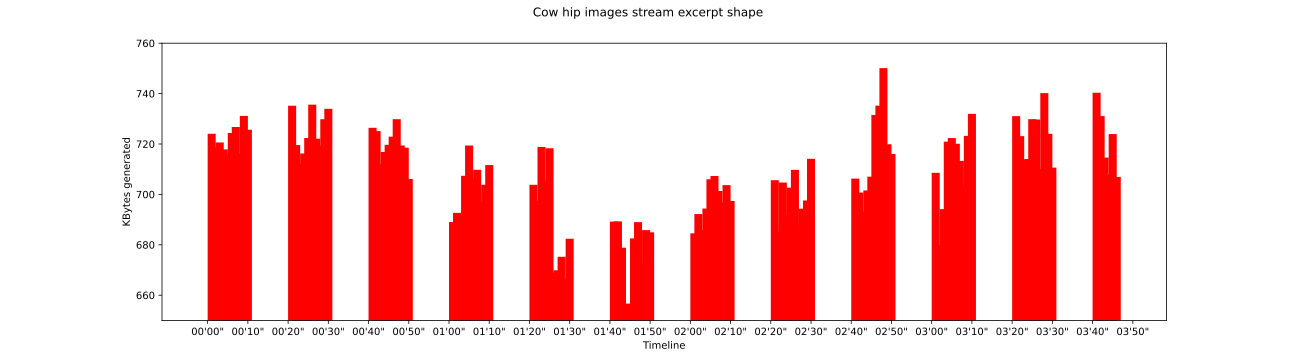
\includegraphics[clip,scale=0.35]{figures/cow_bcs_stream_exerpt}
\par\end{centering}
}
\par\end{centering}
\caption{BCS - workload characterization}
\end{figure}
\begin{figure}
\begin{centering}
\subfloat[street image example\label{fig:street-image-example}]{\includegraphics[scale=0.34]{figures/cycling\lyxdot 2130}

}\subfloat[YoloV4 tiny CNN model benchmarking\label{fig:YoloV4-benchmarking}]{\includegraphics[bb=0bp 36bp 756bp 439.2bp,clip,scale=0.35]{figures/yolov4_tiny_416_tflite_xnnpack_false}

}\\
\subfloat[Street images stream\label{fig:Street-images-stream}]{\begin{centering}
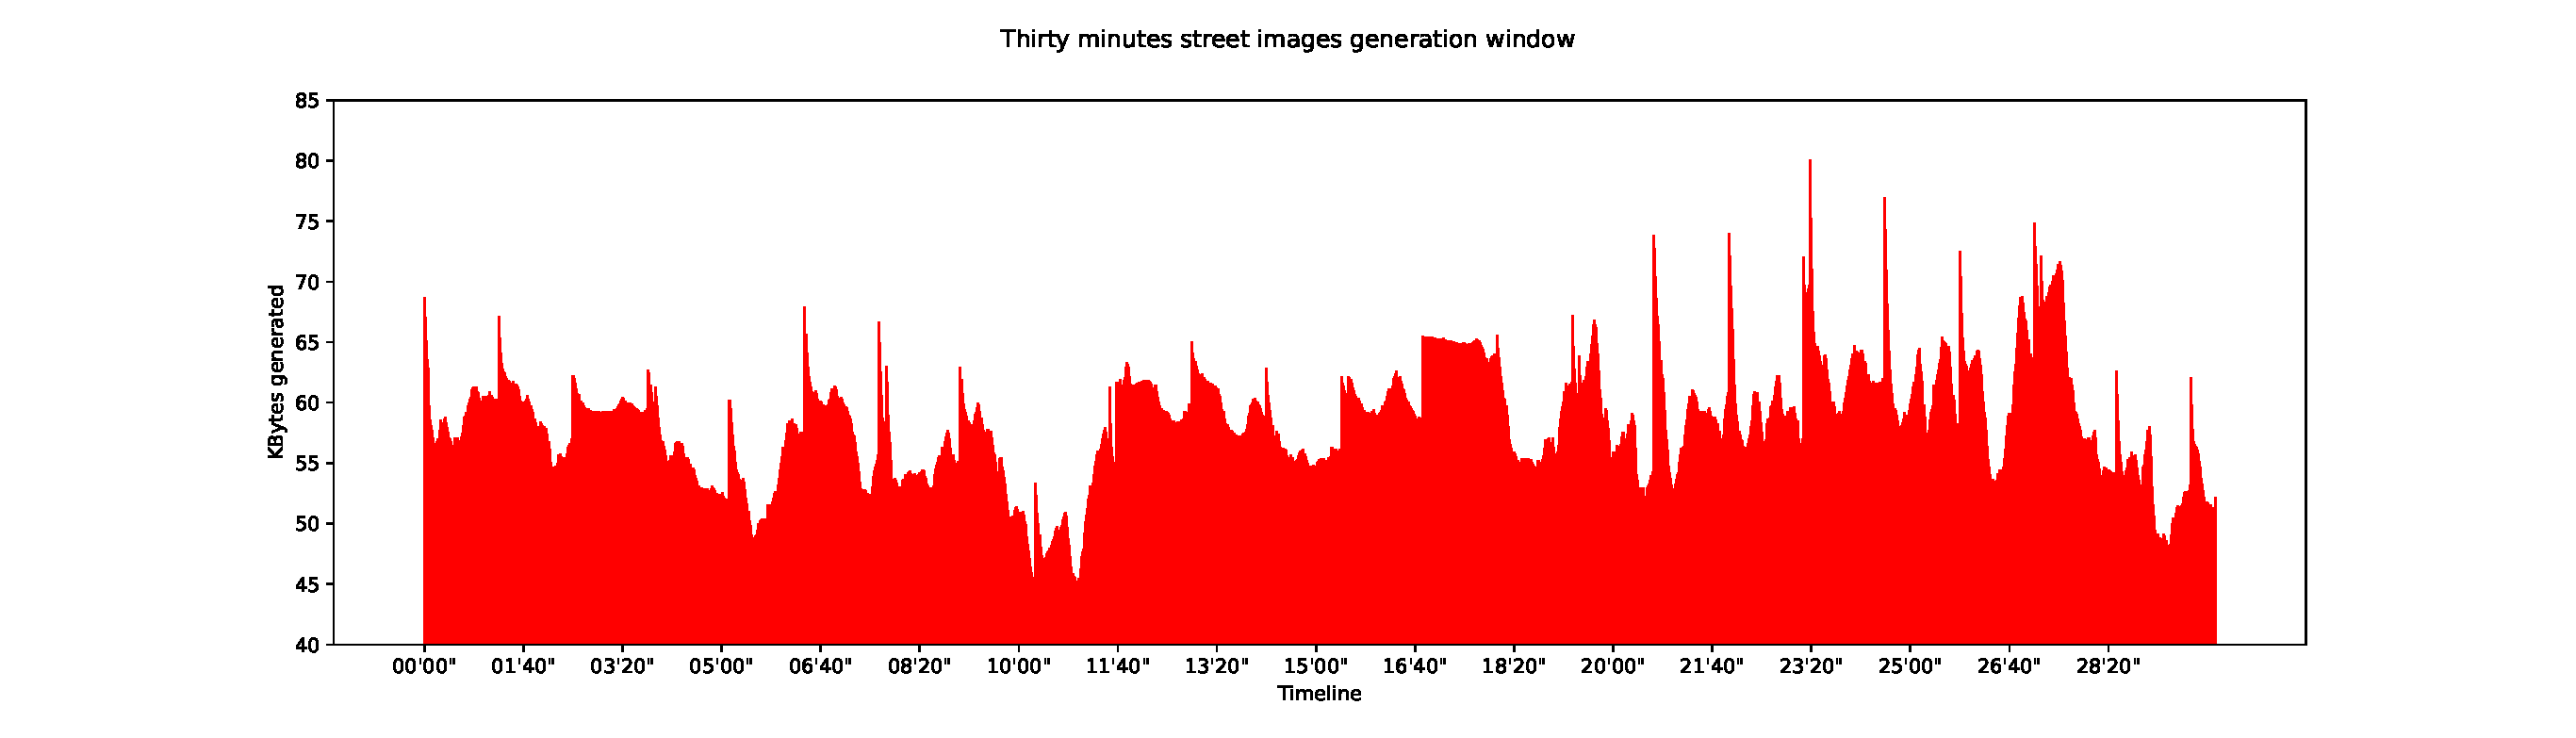
\includegraphics[clip,scale=0.35]{figures/dogs_finder_stream_exerpt}
\par\end{centering}
}~~~~~
\par\end{centering}
\caption{SWT - workload characterization}
\end{figure}
\begin{figure}
\subfloat[Foot image example\label{fig:Foot-image-example-1}]{\includegraphics[bb=0bp 0bp 960bp 1300bp,clip,scale=0.11]{figures/diabetes\lyxdot 157}

}\subfloat[Foot image CNN model benchmarking\label{fig:Foot-Benchmarking}]{\begin{centering}
\includegraphics[bb=0bp 36bp 936bp 439.2bp,clip,scale=0.35]{figures/foot_xnnpack_false}
\par\end{centering}
}\\
\subfloat[Foot images stream\label{fig:Foot-images-stream-1}]{\begin{centering}
\includegraphics[clip,scale=0.35]{figures/diabetes_stream_exerpt}
\par\end{centering}
}

\caption{DMED - workload characterization}
\end{figure}

Irrespective of the application domain, these example application
scenarios present streams with different characteristics not only
by the dynamics of input generation but also the computing capability
required to perform inferences over the input. In addition, it is
assumed that inference results should be available at the master node
with minimun latency, i.e., as close as possible to realtime.

\section{Experiments Setup and Metrics}

For setting up and executing tests we employed a tool set that combines
several open source programs~\cite{mateos2022LiveDewStream,yannibelli2024bagess}
and hardware~\cite{toloza2022motrol} modules. The tool set allow
us to automate tasks involved in experimenting with smartphones and
real workloads including cluster formation, devices preparation (battery
charge/discharge actions), deep learning models deployment, stream
dynamics reproduction, and results collection and summarization.

As discussed earlier in the paper, workloads in edge computing and
IoT scenarios are commonly computed with medium-to-high-end edge nodes
such as SBCs. In the benchmarks we compare performance of several
SBC-based and smartphone-based setups to complete the workloads described
in Section~\ref{sec:workload-characterization}. The ``Edge Setup''
column in Tables~\ref{tab:BCS-Results},\ref{tab:SWT-Results} and
\ref{tab:DMED-Results} differentiates both setups. Considering that
smartphone-based setups comprise clusters of smartphones, Table~\ref{tab:Smartphone-based-setups-details}
expands on the model and battery information of nodes integrating
each cluster. All clusters include a single instance of each smartphone
model. Smartphone brands and models are indicated using a short name
that can be found in Table~\ref{tab:Edge-nodes-features}. The order
in which these short names appear in a row corresponds to the order
in which smartphones' initial battery values appear. The latter were
randomly chosen. Cluster heterogeneity arises from the combination
of smartphones quantity, models and initial battery levels. Cluster
maximum energy and Cluster initial energy, both expressed in Joules,
as well as, Cluster initial battery expressed in \%, all derived from
individual smartphones data, complement the cluster information.

One of the metrics we report is accumulated inference latency, a measure
of how long the makespan deviates from the stream time. The stream
time is the time window where CV tasks are created, while makespan
is the time the inference system employs in completing all the created
CV tasks. Figure~\ref{fig:Inference-accumulated-latency} graphically
represents how these entities coexist in time. Inference completion
of a task naturally occurs in time after the CV task creation. While
tasks creation could occur by following a quite controlled and periodically
process, tasks inference process does not. This is what $\alpha,\beta,\gamma,\delta,\varepsilon,\zeta$
represent in the CV tasks inference timeline associated to each CV
task completion event, i.e. different completion times that could
be given as consequence but not limited to variations in network latency,
CNN data input content and nodes execution capability. When subtracting
stream time to makespan, the result is the accumulated inference latency.
The nearest this difference to zero, the better the setup capability
is to respond with proper inferences time compared to the time taken
to create all CV tasks. A derived metric which gives a notion of the
average time employed by the setup to complete a CV task after a new
CV task is available, could be obtained dividing the accumulated inference
latency by the number of CV tasks created. We call this latter inference
latency. 
\begin{figure}
\centering{}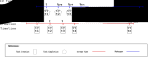
\includegraphics[scale=0.9]{figures/Latency_metric}\caption{Accumulated inference latency: visual explanation\protect\label{fig:Inference-accumulated-latency}}
\end{figure}

Another metric we report is total energy consumption. To measure energy
consumption we followed two approaches depending on the type of setup.
For SBC-based setups we employ a power monitor~\cite{powermeter}
that uses a toroid connected as shown in Figure~\ref{fig:SBC-Power-Monitoring=000020scheme},
which allow us to collect current and voltage readings from an SBC
in a non-invasive way while running workloads. The power monitor is
connected to the 220V AC power and it has a socket after a toroid
where the SBC power source is connected. Current and Voltage readings
are transmitted in realtime via a USB port to a laptop. The power
monitor gives two current and voltage values per second. Then, for
a workload scenario whose inference time is around 3 minutes and 50
seconds, the reported energy consumption is obtained by averaging
460 samples.
\begin{figure}
\begin{centering}
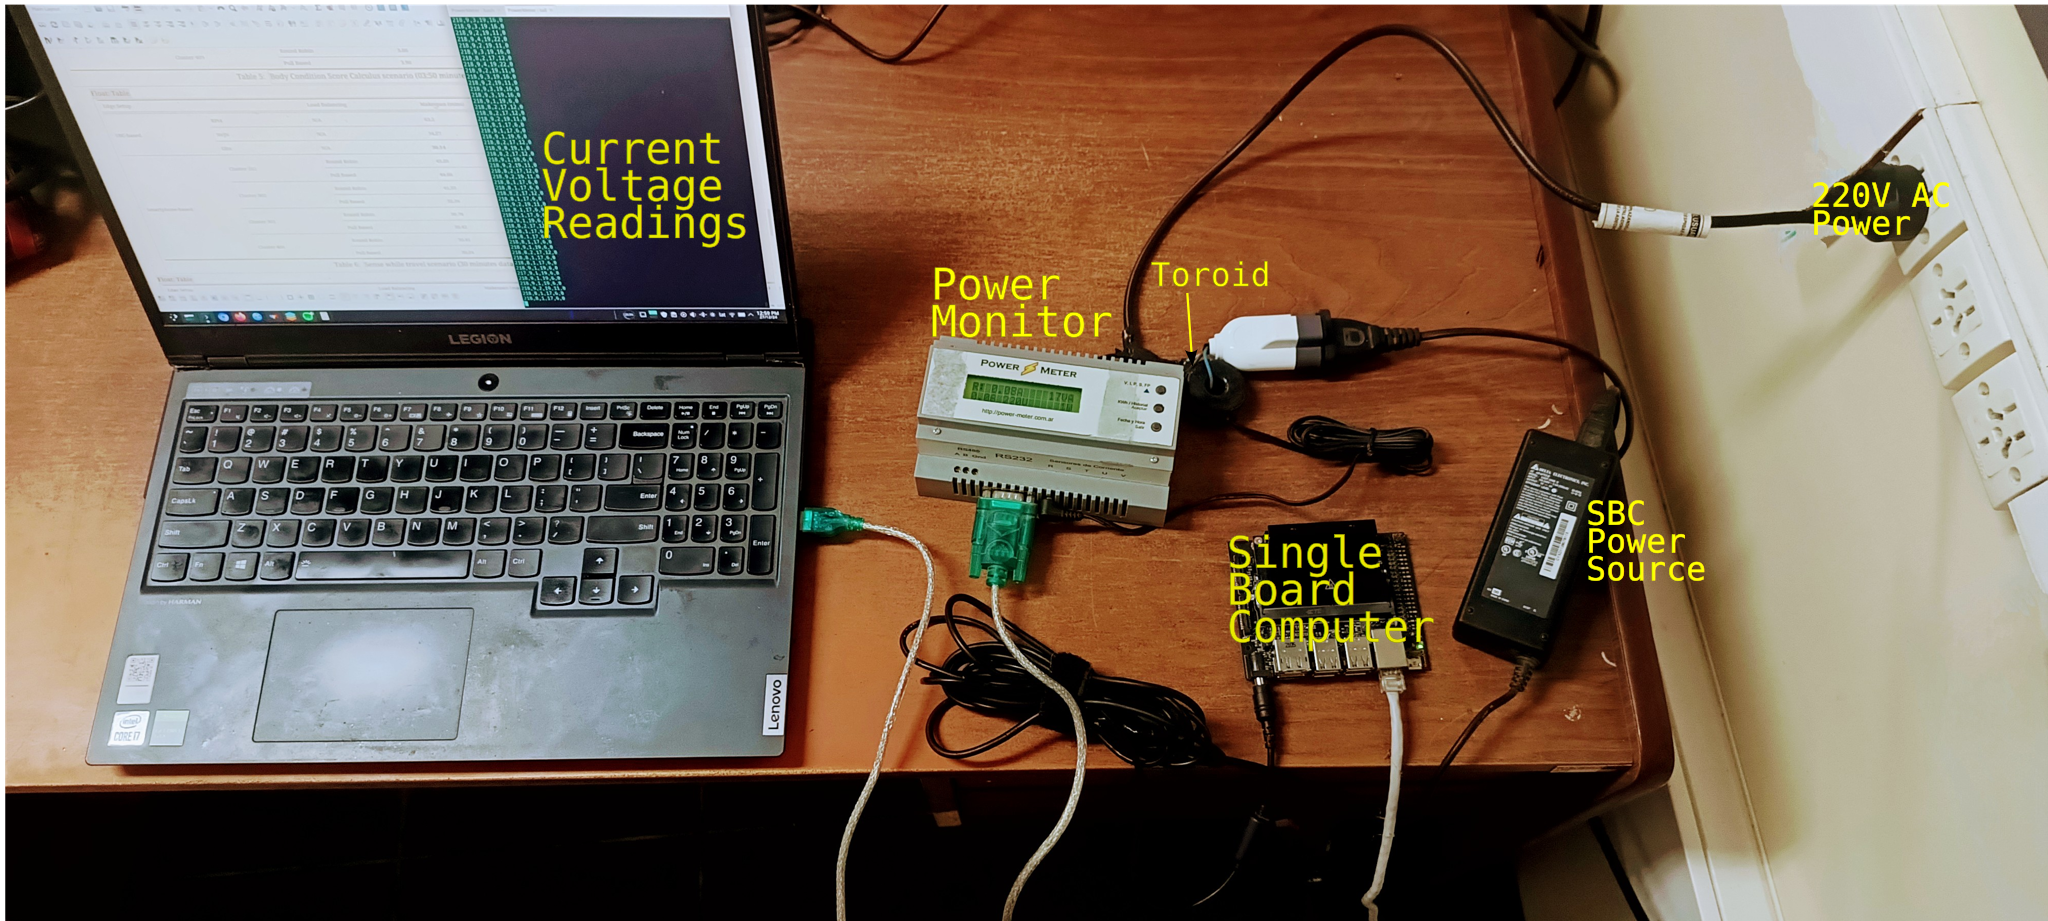
\includegraphics[scale=0.1]{figures/power_meter_labeled}
\par\end{centering}
\caption{SBC power monitoring connection scheme\protect\label{fig:SBC-Power-Monitoring=000020scheme}}
\end{figure}

For smartphone-based setups the described approach for registering
energy consumption cannot be used, because smartphone batteries are
employed as the power source. We, thus, followed a different approachby
registering smartphones battery levels at the beginning and at the
end of a workload scenario. Then, we used battery manufacturer information
-- such as battery mAh and operating voltag e-- of each smartphone
to approximate the total energy used during the workload scenario
execution (WSE), expressed in Joules:
\begin{equation}
WSEJoules=\sum_{i=0}^{\#smartphones}(battLevelDrops^{i}*battMAh^{i}*0.01)*battVoltage^{i}*3.6
\end{equation}

where $\#smartphones$ corresponds to the amount of smartphones integrating
the cluster, $battLevelDrops^{i}$is the amount of battery level drops
registered for the smartphone $i$ used for executing the assigned
workload, which is in turn calculated as: 
\begin{equation}
battLevelDrops=batt_{endWSE}-batt_{startWSE}
\end{equation}

where $batt_{startWSE}$ and $batt_{endWSE}$ are the battery level
of smartphone $i$ at the start and end of the workload scenario execution
respectively, $battMah^{i}$ and $battVoltage^{i}$ are milli-amperes
hour and operating voltage information respectively, provided by the
battery manufacturer of smartphone $i$. Formula~1 emerges from combining
a rule of three that relates battery percentage usage with the unit
conversion formula from mAh to Joules which is $mAh*voltage*3.6=JoulesOfenergy$.

Additionally, since a workload scenario execution using smartphone-based
setups might cause different battery percentage usage on each node,
we report Jain's fairness index~\cite{jain1984quantitative} as a
metric that summarizes intra-cluster energy utilization. In other
words, the metric is used to measure the disparity of energy pulled
by the system from resource provider nodes. The metric takes values
from 0 to 1. The nearest the index to value of one the more balanced
the energy utilization among cluster nodes is. The Jain's index inspired
formula we applied is:

\begin{equation}
Fairness=\frac{\left[\sum_{i=0}^{\#smartphones}battLevelDrops^{i}\right]^{2}}{\#smartphones*\left(\sum_{i=0}^{\#smartphones}\left[(battLevelDrops^{i})\right]^{2}\right)}
\end{equation}

Since all smartphone-based setups comprise clusters of at least two
heterogeneous smartphones, it was necessary to indicate the load balancing
strategy used to distribute load between these. For this reason, all
smartphone-based setups are indicated with Round Robin or Pull-Based
as value in the load balancing column. Round Robin is a classic load
balancing strategy that assigns an incoming task to the next available
node using a rotating scheme, ensuring workload is evenly distributed
among all participating devices. By contrast, with a Pull-Based approach
tasks are pulled by nodes from a shared queue based on their availability.
In our configurations, cluster nodes were configured to pull at most
one task per request. In turn, a node is able to make a request when
the result of the previously pulled task was sent back to the Edge
master, i.e. the task is marked by the system as completed.

\begin{table}
\begin{centering}
\begin{tabular}{l>{\raggedright}p{0.04\columnwidth}>{\raggedright}p{0.27\columnwidth}>{\raggedright}p{0.12\columnwidth}>{\raggedright}p{0.07\columnwidth}>{\raggedright}p{0.07\columnwidth}>{\raggedright}p{0.07\columnwidth}}
\toprule 
\multirow{1}{*}{{\scriptsize Cluster ID}} & \multirow{1}{0.04\columnwidth}{{\scriptsize Cluster size}} & {\scriptsize Smartphone models} & \multirow{1}{0.12\columnwidth}{{\scriptsize Smartphones initial battery \%}} & {\scriptsize Cluster initial energy (Joules)} & {\scriptsize Cluster max. energy (Joules)}{\scriptsize\tablefootnote{To calculate this value we used a formula derived from formula 1 assuming
each smartphone is fully charged.}} & {\scriptsize Cluster initial battery \%}{\scriptsize\tablefootnote{The value was calculated using formula 1, replacing batteryDrops by
battery level of each smartphone at the begining of a workload test.}}\tabularnewline
\midrule
{\scriptsize Cl202} & {\scriptsize 2} & {\scriptsize XRN7, MotG9} & {\scriptsize 87, 75} & {\scriptsize 99532.80} & {\scriptsize 123840} & {\scriptsize 80.37}\tabularnewline
{\scriptsize Cl203} & {\scriptsize 2} & {\scriptsize XRN7, MotG9} & {\scriptsize 27, 54} & {\scriptsize 51904.80} & {\scriptsize 123840} & {\scriptsize 41.91}\tabularnewline
{\scriptsize Cl205} & {\scriptsize 2} & {\scriptsize MotG9, SamA30} & {\scriptsize 54, 30} & {\scriptsize 53152.20} & {\scriptsize 122454} & {\scriptsize 43.41}\tabularnewline
{\scriptsize Cl301} & {\scriptsize 3} & {\scriptsize SamA30, XRN7, MotG9} & {\scriptsize 27, 45, 60} & {\scriptsize 80582.58} & {\scriptsize 177894} & {\scriptsize 45.30}\tabularnewline
{\scriptsize Cl302} & {\scriptsize 3} & {\scriptsize SamA30, SamA02, MotG9} & {\scriptsize 27, 45, 60} & {\scriptsize 86195.88} & {\scriptsize 190368} & {\scriptsize 45.28}\tabularnewline
{\scriptsize Cl304} & {\scriptsize 3} & {\scriptsize MotG6, XRN7, MotG9} & {\scriptsize 77, 25, 53} & {\scriptsize 81712.80} & {\scriptsize 164880} & {\scriptsize 49.55}\tabularnewline
{\scriptsize Cl305} & {\scriptsize 3} & {\scriptsize MotG9, MotG6, SamA30} & {\scriptsize 54, 92, 25} & {\scriptsize 88206.30} & {\scriptsize 163494} & {\scriptsize 53.95}\tabularnewline
{\scriptsize Cl408} & {\scriptsize 4} & {\scriptsize MotG6, SamA30, XRN7, MotG9} & {\scriptsize 30, 27, 45, 60} & {\scriptsize 92894.58} & {\scriptsize 218934} & {\scriptsize 42.43}\tabularnewline
{\scriptsize Cl409} & {\scriptsize 4} & {\scriptsize MotG6, SamA30, XRN7, MotG9} & {\scriptsize 88, 80, 38, 49} & {\scriptsize 133941.6} & {\scriptsize 218934} & {\scriptsize 61.18}\tabularnewline
{\scriptsize Cl411} & {\scriptsize 4} & {\scriptsize MotG6, SamA30, XRN7, MotG9} & {\scriptsize 25, 52, 44, 38} & {\scriptsize 88753.68} & {\scriptsize 218934} & {\scriptsize 40.54}\tabularnewline
\bottomrule
\end{tabular}
\par\end{centering}
\caption{Details of the smartphone-based setups\protect\label{tab:Smartphone-based-setups-details}}

\end{table}


\subsection{Benchmark Results\protect\label{subsec:Benchmark-results}}

\subsubsection{Performance Analysis}

\begin{figure}
\begin{centering}
\includegraphics[scale=0.6]{figures/performance}
\par\end{centering}
\caption{Accumulated Inference Latency for the three scenarios. For the cluster
setups, we indicate the load balancing technique used (PB=pull based;
RR=round robin). Load balancing is not used in SBC-based setups.\protect\label{fig:Accumultated-Inference-Latency}}

\end{figure}
Figure~\ref{fig:Accumultated-Inference-Latency} shows the performance
achieved by all setups for all scenarios. Blue bars correspond to
SBC-based setups while orange ones to smartphone-based setups. By
comparing all setups, it can be clearly noted that the best performance,
i.e. the lowest accumulated inference latency value in all tested
scenarios is achieved with the Gigabyte Brix setup. The close-to-zero
value indicates that inferences performed with this setup is near
to real-time, i.e. inference results associated to all CV tasks are
obtained within the stream time. Concretely, in the BCS scenario,
the accumulated latency in a stream time of 3' 50'' was 3 seconds.
In the SWT scenario, the accumulated latency in a stream time of 30'
was 1.2 seconds while in the DMED scenario with a stream time of 8'55'',
the value was 3.6 seconds. With the Raspberry Pi4 and Nvidia Jetson
Nano setups the obtained accumulated inference latency was significantly
greater, and in most cases, the inference latency was the stream time
multiplied by a factor of two to four -- for detailed values please
refer to tables in appendix~\ref{sec:Appendix-A} -- . The Nvidia
Jetson nano setups performed better than the Raspberry Pi4 setups
in all cases. However, the workload always exceeded the inference
capability. With these setups, reducing workload would be necessary
to achieve near real-time performance. Some alternatives to reduce
workload are creating more lightweight CV tasks by dropping frames
and/or offloading some CV tasks to other Edge nodes. These alternatives
could come, in turn, with some QoS degradation due to increased network
latency.

When comparing smartphone-based setups for the BCS scenario, we empirically
confirm what other studies found~\cite{hu2019deephome,huang2021enabling}:
by incrementing the number of participating smartphones, performance
improves, i.e, lower accumulated inference latency is obtained. This
is also true for the SWT and DMED scenarios. However, not only the
number of smartphones impact the setup inference service capability,
but also the smartphones computing characteristics. Clusters 301 and
302, for instance, are of the same size. Both clusters are composed
by the Samsung A30 and the Motorola Moto G9 play. However, the Samsung
A02 smartphone present in Cluster 302 is not present in Cluster 301,
which has the Xiaomi Redmi Note 7 instead. If we compare the inference
times associated to the latter mentioned smartphone models and reported
in Figures~\ref{fig:Cow-BCS-Benchmarking},\ref{fig:YoloV4-benchmarking}
and \ref{fig:Foot-Benchmarking}, we note that the computing capability
of the Samsung A02 is in between 2.62 and 3.99 times slower than that
of the Xiaomi Redmi Note 7. The effect of such difference is observed
in the performance values registered for the SWT scenario, where both
clusters are tested. While the accumulated inference latency with
Cluster 301 was between $\backsim$16 and $\backsim$31 seconds, with
Cluster 302 it was between $\backsim$131 and $\backsim$678 seconds.

Another observation when comparing smartphone-based setups is that
in general pull-based load balancing scheme achieves lower accumulated
inference latency than round robin. This is because using pull-based
allow the cluster to balance the workload in accordance to the availability
and computing capability of worker nodes rather than treat all nodes
with the same capability as round robin does. This advantage of pull-based
over round robin diminishes in clusters where nodes present quite
similar computing capability, which is the case of Cluster 202 in
the SWT scenario, or even when computing resources are apparently
abundant enough to satisfy the workload requirements, which seems
to be the case of Cluster 408. In general, the most competitive accumulated
inference latency comparison to that obtained by the Gigabyte Brix
setup was always achieved with a pull-based load balancing scheme.
For example, in the BCS scenario, the difference between Cluster 409
and Gigabyte Brix setups was less than 8 seconds. The third best performance
was also achieved with a pull-based setup. The Cl304-PB, a size 3
cluster, achieves quite similar performance to that of a size cluster
4 combined with round robin, i.e. Cl409-RR. A similar analysis is
valid in the SWT and DMED scenarios, with Clusters 408 and 411 respectively.
Pull-based load balancing scheme achieves considerable better performance
than round robin when clusters nodes present heterogeneous computing
capabilities or when available computing capabilities are tight to
cope with realtime tasks requirements.

\subsubsection{Energy Consumption-Performance Tradeoff Analysis}

In view of the high energy consumption that AI applications already
demand and expected further increases, studies in this regard~\cite{henderson2020Towards,strubell2020energy,garcia2019estimation}
and initiatives such as the Low-Power Recognition Challenge~\cite{gauen2017low}
encourage the improvement of not only DLs model's performance but
also the energy its execution and training consume. In this sense,
we study the tradeoff between performance and energy consumed in all
evaluated scenarios. Figure~\ref{fig:Energy-consumption-Performance-tradeoff}
reports the energy consumption and accumulated inference latency tradeoff
between different setups in each tested scenario. The best setups
are those that achieve the minimum accumulated inference latency using
the least energy, i.e., those positioned close to the origin. As can
be observed, in all scenarios the best balance is always achieved
by orange dots with a label starting with Cl which corresponds to
smartphone-based setups. It can be noted, for instance, that the accumulated
inference latency of GBx setups are the lowest in BCS, SWT and DMED
scenarios, however, these are also associated to the highest values
of energy utilization. Moreover, the slowest setups are not necessary
associated to the most convenient ones in terms of energy consumption.
Interestingly, smartphone-based setups, particularly four-node clusters
using pull-based as load balancing scheme offer a good tradeoff in
all scenarios, i.e. competitive performance with the least energy
consumption. These are the cases of Cl409-PB, Cl408-PB and Cl411-PB
for BCS, SWT and DMED scenarios respectively. In other words, for
the BCS scenario, when it is acceptable that all CV tasks results
were calculated with a delay of 7.8 seconds w.r.t to the fastest setup,
the Cluster 409 setup with pull-based scheme can achieve the same
objective by utilizing $\backsim$1510 Joules, i.e. almost three times
less energy than the Gigabyte Brix setup. Similar relations can be
found for the SWT and DMED scenarios.

\begin{figure}
\begin{centering}
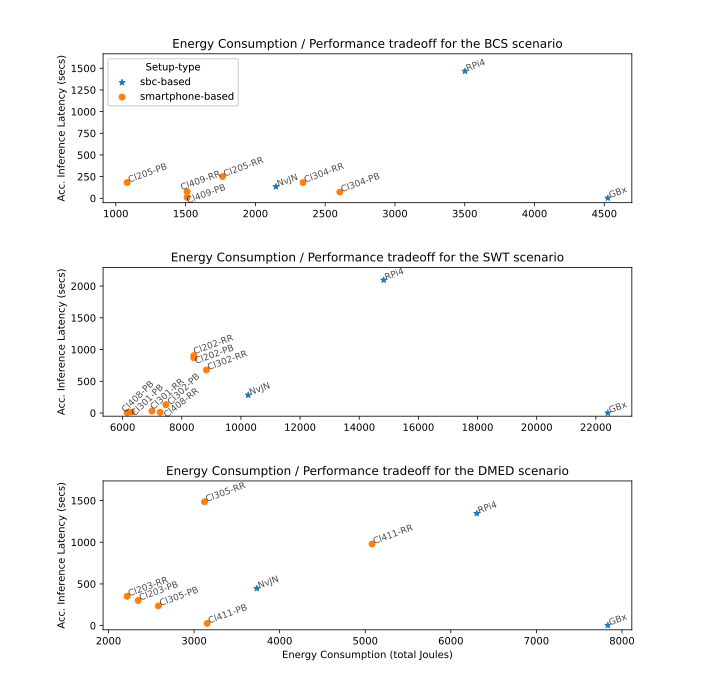
\includegraphics[bb=50bp 0bp 1000bp 961bp,clip,scale=0.7]{figures/energy-performance-tradeoff}
\par\end{centering}
\caption{Energy consumption / Performance tradeoff\protect\label{fig:Energy-consumption-Performance-tradeoff}}

\end{figure}


\subsubsection{Battery Utilization Analysis}

For smartphone-based setups, it is relevant to show the impact of
CV tasks computation on clusters energy availability. Provided that
clusters are composed of at least two nodes, cluster battery can be
seen as the aggregation of nodes battery. To represent the cluster
current battery level with a single positive integer value, we aggregate
the Joules each smartphone contributes to the global cluster energy.
By assuming that a cluster with 100\% global battery level is one
where batteries of all integrating smartphones are fully charged,
using Equation~1 it is possible to calculate the global battery level
expressed in percentage of a cluster for different smartphones battery
levels. Then, Figure~\ref{fig:Global-battery-impact} shows global
battery level drops for all smartphone-based setups evaluated in all
scenarios. Since in all cases smartphone-based setups run workloads
while unplugged from the electricity grid, i.e. with batteries in
discharging mode, the battery drops were calculated as the difference
between the initial and the final global battery level of a cluster
before and after the workload execution respectively. In Figure~\ref{fig:Global-battery-impact}
it can be noted, for instance, that CV tasks in the SWT scenario causes
the highest global battery drops compared to BCS and DMED, which is
mainly due to the length of the workload execution -30' compared to
$\backsim$4' and $\backsim$9' in BCS and DMED respectively.

Another observation that emerges from Figure~\ref{fig:Global-battery-impact}
is that when comparing cluster battery level drops between clusters
w.r.t. the same scenario, it appears to decrease as cluster size increases.
In fact, as more smartphones integrate a cluster the cluster battery
also increases and one percentage of such cluster battery is represented
by a larger number in Joules. Something similar happens when two clusters
are of the same size but one has smartphones whose batteries have
more energy capacity than the other, which is the case of Cl301 and
Cl302. However, a cluster with a bigger battery does not imply that
it will complete tasks in a more energy-efficient way. As an example,
refer to the ``Max. Cluster Energy'' column of Table~ \ref{tab:Smartphone-based-setups-details}
to appreciate that Cl302 has slightly larger cluster battery capacity
than Cl301, because the Xiaomi RN7 with a battery capacity of 4000
mAh in Cl301 was swapped by the Samsung A02 with a battery capacity
of 4900 mAh in Cl302. However, according to Figure~\ref{fig:YoloV4-benchmarking},
the latter smartphone is almost four times slower to perform a task
from the SWT scenario than the former, meaning that Cl302 will spent
more energy than Cl301 in completing the same amount of tasks. This
explains why despite having a larger cluster battery, the battery
drop of Cl302 is larger than that of Cl301 in SWT scenario shown in
Figure~\ref{fig:Global-battery-impact}. Moreover, it is relevant
to point out that, in general, the pull-based load balancing scheme
achieves equal or less global battery drops than round robin (approximately
0.5\%). 
\begin{figure}
\centering{}\subfloat[Global battery impact\label{fig:Global-battery-impact}]{\begin{centering}
\includegraphics[scale=0.5]{figures/cluster_consumed_battery}
\par\end{centering}
}~\subfloat[Fairness index\label{fig:Fairness-index}]{\begin{centering}
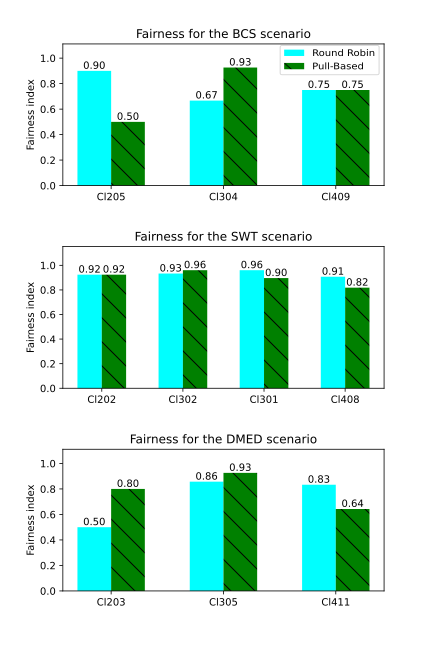
\includegraphics[scale=0.5]{figures/fairness}
\par\end{centering}

}\caption{CV tasks impact on clusters global energy availability and Fairness
index\protect\label{fig:clusters-energy-availability}}
\end{figure}

Finally, we analyze fairness values derived from applying the round
robin and the pull-based load balancing schemes. The index serves
as a hint on how the edge cluster utilizes energy from all participating
smartphones. The more the value approximates to one, the more balanced
the battery utilization is. Figure~\ref{fig:Fairness-index} reveals
that in some clusters, the pull-based scheme achieves slightly higher
fairness values than that of round robin, while in other cases, the
results are the opposite. There are cases where even both schemes
achieve equal fairness values. Since there is not a clear pattern,
we can conclude that there is not a clear winner load balancing scheme
as measured by the fairness index.

\section{Discussion}

A few previous works have also focused on proving the strengths of
edge computing for reducing end-to-end latency and allowing the execution
of data intensive IoT and delay sensitive applications~\cite{yi2017lavea,kang2017neurosurgeon}.
In this work, we explored how edge computing capabilities can be augmented
with smartphone clusters under different workload scenarios for real-time
AI inferences involving image streams. The competitive performance
and reduced energy consumption that smartphone clusters showed, along
with the pervasiveness of such devices worldwide evidence their suitability
for being considered a powerful harness to complement in-the-field,
already present edge settings, and/or to fully support opportunistic
distributed inference in a sustainable form. However, there are several
questions still open, demanding for further research. One of these
relates to whether current software stacks including middlewares for
distributed computing~\cite{torres2021open,tuli2019edgelens} and
frameworks for AI execution~\cite{guo2019empirical} in low-powered
devices are prepared to integrate smartphone clusters as a new type
of edge node by attending diverse aspects related to computational
resource provision with devices that present non-dedicated resources,
i.e. with user applications that have high priority on the usage of
resources, unstable communication due to device's owner physical position
changes, and resource scavenging time limited by batteries operation
time. 

Another open question concerns incentives that make a device's onwer
to offer unused computing mobile resources. In the literature, it
has been identified at least two schemes. One of them is associated
to altruistic attitudes of devices owners, in some sense, similar
to what is promoted in volunteer computing platforms with unused computing
cycles of desktop computers for scientific projects. Only that, in
this case, targeting daily normal situations that required in-the-field
inference capability either for reducing cost of data transmission
-e.g. chronic disease health monitoring-, complement safety-guard
mechanisms in risky situations -e.g., alerting about obstacles in
the road while driving-, providing realtime response to improve user
experience - e.g., augmented reality applications in tourism-related
activities- among others. By contrast, the other incentive scheme
we visualize is based on a opportunistic inference as a service approach
that benefits device's owner with some revenue in the form of credits~\cite{chatzopoulos2017flopcoin}
or reputation~\cite{chatzopoulos2016openrp}, in exchange of completing
tasks that require in-the-field inference capability, for example,
as a complement to surveillance cameras for crime prevention in public
spaces. The energy consumption caused by using efficient hardware
such as that embedded in smartphones w.r.t using other edge nodes
can be used as baseline for establishing economically and environmentally
sustainable inference mechanisms.

In this regard, another aspect worth to be mentioned that is intimately
related to AI and computing infrastructures concerns energy consumption
and hence, indirectly, CO2 emissions. In its World Energy Outlook
2024~\cite{IEAReports,IEAElect2024}, the well-known International
Energy Agency (IEA), projects that energy consumption in datacenters
is set to expand in the future, in part due to digitalization of the
economy but also as a consequence of the rapid advance of AI technologies
and the outbreak of AI startups. In fact, figures from 2022 also reported
by the IEA -i.e. even some years before the AI boom we have been experiencing
since then- result in datacenters consuming 1-2\% of the world\textquoteright s
electricity, which is backed up by estimates from similar studies~\cite{masanet2020recalibrating,malmodin2024ict}.
This positions energy-efficient approaches to edge computing as a
crucial path to cap these estimates while providing viable computing
settings to continue helping bringing AI to the masses. Then, edge
computing research should not only merely quantify energy savings
compared to traditional computing approaches but also develop mechanisms
to measure the impact on CO2 emissions at the software level such
as~\cite{schmidt2024carbond}. Quantification must also consider
current mobile hardware manufacturing practices, for example promoting
replaceable (sealed) batteries, which encourage users to upgrade to
a new device when battery performance declines, rather than simply
replacing the battery. Metrics such as the Software Carbon Intensity
(SCI) index~\cite{SoftwareCarbonIntensity} might serve as a pertinent
reference since it captures the environmental impact of software in
terms of CO2 emissions considering carbon intensity of the energy
used to run software and the embedded emissions due to the carbon
footprint to build the hardware on which the software runs.

\section{Conclusions and Future Works\protect\label{sec:Conclusions-and-future}}

In this work, we explored the computing capabilities of mobile distributed
computing setups for real-time inferences by experimenting with heterogeneous
AI workloads, built upon real convolutional neural network (CNN) models
and images data sets that were used to emulate computer vision (CV)
tasks generated in a stream-like fashion. We run and compare the performance
achieved by several setups built with commodity hardware including
single board computers (SBCs) and smartphone clusters that could be
found or exploited in practical Edge computing and IoT application
scenarios.

We conclude that tiny clusters composed by two to four low to middle-end
smartphones using a pull-based load balancing scheme offer competitive
performance compared to an SBC equipped with a reasonable CPU (Intel
core i5 8th generation) in computing realtime inferences of CV tasks.
This suggests that to satisfy certain delay sensitive application
scenarios, the exploitation of already-in-place smartphones clusters
can be considered before the investment and deployment of SBCs. According
to Table~\ref{tab:Edge-nodes-features} the necessary investment
for supporting the evaluated scenarios using a powerful SBC like the
Gigabyte Brix is only 30\% cheaper than with a cluster-based setup
of four low to mid-end smartphones. This is when not considering that
smartphones can be already present in the application context and
the computing capability hired to device owners. In any case, energy
consumption measurements show that the tradeoff including performance
and energy consumption favors smartphone clusters over SBCs. The former
can deliver competitive performance with a reduction of around tree
times the energy consumption spent by a powerful SBC such as the Gigabyte
Brix.

Several improvement opportunities lend itself to future work. In line
with developing new load balancing heuristics, and based on the results
from preliminary runs, we plan to improve previously published heuristics
that use MFLOPs to rank nodes computing capabilities~\cite{hirsch2021task}.
An alternative solution is to use information derived from the Tensorflow
benchmarking tool~\cite{tensorflowBenchmarking}. In spite of differences
observed in inference times obtained via the Tensorflow benchmarking
tool and results collected in experiments using real input, relative
benchmarked positions between edge nodes are similar, meaning that
it is feasible to use such tool to build node rankings that serve
as input for the load balancing component to distribute tasks based
on an alternative nodes performance score to the classic MFLOPs. 

Another future direction is to consider other forms of workload distributions,
i.e. that exploit the structure of deep learning (DL) arquitectures,
for example, split computing, early exiting techniques, and model
quantization~\cite{chen2020deep} to better exploit CPU capabilities
of mobile platforms while performing network inferences.

\section*{Acknowledgments}

This work was funded by CONICET via grants PIBAA-28720210101298CO
and PIP-11220210100138CO.

\bibliographystyle{plain}
\bibliography{references-tidy}


\section*{Appendix A\protect\label{sec:Appendix-A}}

Tables~\ref{tab:BCS-Results}, \ref{tab:SWT-Results} and \ref{tab:DMED-Results}
contain the data reported in all graphs presented in Section~\ref{subsec:Benchmark-results}
for BCS, SWT and DMED scenarios.

\begin{table}
\begin{centering}
\begin{tabular}{>{\raggedright}p{0.09\paperwidth}>{\raggedright}p{0.09\paperwidth}>{\raggedright}p{0.1\paperwidth}>{\raggedright}p{0.07\paperwidth}>{\raggedright}p{0.07\paperwidth}>{\raggedright}p{0.07\paperwidth}>{\raggedright}p{0.07\paperwidth}}
\toprule 
\multicolumn{2}{l}{{\scriptsize Edge Setup}} & {\scriptsize Load Balancing} & {\scriptsize Acc. Inference Latency (secs)} & {\scriptsize Jain's Fairness Index} & {\scriptsize Cluster Consumed Battery (\%)} & {\scriptsize Consumed Energy (Joules)}\tabularnewline
\midrule
\midrule 
\multirow{3}{0.09\paperwidth}{{\scriptsize SBC-based}} & {\scriptsize RPi4} & {\scriptsize N/A} & {\scriptsize 1467} & {\scriptsize N/A} & {\scriptsize N/A} & {\scriptsize 3501.97}\tabularnewline
\cmidrule{2-7}
 & {\scriptsize NvJN} & {\scriptsize N/A} & {\scriptsize 134.4} & {\scriptsize N/A} & {\scriptsize N/A} & {\scriptsize 2147.13}\tabularnewline
\cmidrule{2-7}
 & {\scriptsize GBx} & {\scriptsize N/A} & {\scriptsize\textbf{3.0}} & {\scriptsize N/A} & {\scriptsize N/A} & {\scriptsize 4524.82}\tabularnewline
\midrule 
\multirow{6}{0.09\paperwidth}{{\scriptsize Smartphone-based}} & \multirow{2}{0.09\paperwidth}{{\scriptsize Cluster 205}} & {\scriptsize Round Robin} & {\scriptsize 251.4} & {\scriptsize 0.9} & {\scriptsize 1.44} & {\scriptsize 1765.08}\tabularnewline
\cmidrule{3-7}
 &  & {\scriptsize Pull Based} & {\scriptsize 181.7} & {\scriptsize 0.5} & {\scriptsize 0.88} & {\scriptsize 1081.08}\tabularnewline
\cmidrule{2-7}
 & \multirow{2}{0.09\paperwidth}{{\scriptsize Cluster 304}} & {\scriptsize Round Robin} & {\scriptsize 181.8} & {\scriptsize 0.667} & {\scriptsize 1.42} & {\scriptsize 2341.29}\tabularnewline
\cmidrule{3-7}
 &  & {\scriptsize Pull Based} & {\scriptsize 71.4} & {\scriptsize 0.926} & {\scriptsize 1.58} & {\scriptsize 2605.10}\tabularnewline
\cmidrule{2-7}
 & \multirow{2}{0.09\paperwidth}{{\scriptsize Cluster 409}} & {\scriptsize Round Robin} & {\scriptsize 76.2} & {\scriptsize 0.750} & {\scriptsize 0.69} & {\scriptsize 1510.64}\tabularnewline
\cmidrule{3-7}
 &  & {\scriptsize Pull Based} & {\scriptsize 10.8} & {\scriptsize 0.750} & {\scriptsize 0.69} & {\scriptsize 1510.64}\tabularnewline
\bottomrule
\end{tabular}
\par\end{centering}
\caption{Body Condition Score scenario (03:50 minutes data stream)\protect\label{tab:BCS-Results}}
\end{table}

\begin{table}
\begin{centering}
\begin{tabular}{>{\raggedright}p{0.09\paperwidth}>{\raggedright}p{0.09\paperwidth}>{\raggedright}p{0.1\paperwidth}>{\raggedright}p{0.07\paperwidth}>{\raggedright}p{0.07\paperwidth}>{\raggedright}p{0.07\paperwidth}>{\raggedright}p{0.07\paperwidth}}
\toprule 
\multicolumn{2}{l}{{\scriptsize Edge Setup}} & {\scriptsize Load Balancing} & {\scriptsize Acc. Inference Latency (secs)} & {\scriptsize Jain's Fairness Index} & {\scriptsize Cluster Consumed Battery (\%)} & {\scriptsize Consumed Energy (Joules)}\tabularnewline
\midrule
\midrule 
\multirow{3}{0.09\paperwidth}{{\scriptsize SBC-based}} & {\scriptsize RPi4} & {\scriptsize N/A} & {\scriptsize 2094.6} & {\scriptsize N/A} & {\scriptsize N/A} & {\scriptsize 14827.11}\tabularnewline
\cmidrule{2-7}
 & {\scriptsize NvJN} & {\scriptsize N/A} & {\scriptsize 282.6} & {\scriptsize N/A} & {\scriptsize N/A} & {\scriptsize 10246.13}\tabularnewline
\cmidrule{2-7}
 & {\scriptsize GBx} & {\scriptsize N/A} & {\scriptsize\textbf{1.2}} & {\scriptsize N/A} & {\scriptsize N/A} & {\scriptsize 22403.73}\tabularnewline
\midrule 
\multirow{8}{0.09\paperwidth}{{\scriptsize Smartphone-based}} & \multirow{2}{0.09\paperwidth}{{\scriptsize Cluster 202}} & {\scriptsize Round Robin} & {\scriptsize 903.6} & {\scriptsize 0.924} & {\scriptsize 6.79} & {\scriptsize 8408.74}\tabularnewline
\cmidrule{3-7}
 &  & {\scriptsize Pull Based} & {\scriptsize 869.4} & {\scriptsize 0.924} & {\scriptsize 6.79} & {\scriptsize 8408.74}\tabularnewline
\cmidrule{2-7}
 & \multirow{2}{0.09\paperwidth}{{\scriptsize Cluster 302}} & {\scriptsize Round Robin} & {\scriptsize 678.0} & {\scriptsize 0.933} & {\scriptsize 4.64} & {\scriptsize 8833.07}\tabularnewline
\cmidrule{3-7}
 &  & {\scriptsize Pull Based} & {\scriptsize 131.4} & {\scriptsize 0.960} & {\scriptsize 3.92} & {\scriptsize 7462.43}\tabularnewline
\cmidrule{2-7}
 & \multirow{2}{0.09\paperwidth}{{\scriptsize Cluster 301}} & {\scriptsize Round Robin} & {\scriptsize 31.2} & {\scriptsize 0.960} & {\scriptsize 3.93} & {\scriptsize 6991.23}\tabularnewline
\cmidrule{3-7}
 &  & {\scriptsize Pull Based} & {\scriptsize 16.2} & {\scriptsize 0.896} & {\scriptsize 3.54} & {\scriptsize 6297.45}\tabularnewline
\cmidrule{2-7}
 & \multirow{2}{0.09\paperwidth}{{\scriptsize Cluster 408}} & {\scriptsize Round Robin} & {\scriptsize 10.8} & {\scriptsize 0.907} & {\scriptsize 3.32} & {\scriptsize 7268.61}\tabularnewline
\cmidrule{3-7}
 &  & {\scriptsize Pull Based} & {\scriptsize 6.0} & {\scriptsize 0.818} & {\scriptsize 2.81} & {\scriptsize 6152.04}\tabularnewline
\bottomrule
\end{tabular}
\par\end{centering}
\caption{Sense while travel scenario (30 minutes data stream)\protect\label{tab:SWT-Results}}
\end{table}
\begin{table}
\begin{centering}
\begin{tabular}{>{\raggedright}p{0.1\paperwidth}>{\raggedright}p{0.1\paperwidth}>{\raggedright}p{0.1\paperwidth}>{\raggedright}p{0.07\paperwidth}>{\raggedright}p{0.07\paperwidth}>{\raggedright}p{0.07\paperwidth}>{\raggedright}p{0.07\paperwidth}}
\toprule 
\multicolumn{2}{l}{{\scriptsize Edge Setup}} & {\scriptsize Load Balancing} & {\scriptsize Acc. Inference Latency (secs)} & {\scriptsize Jain's Fairness Index} & {\scriptsize Cluster Consumed Battery (\%)} & {\scriptsize Consumed Energy (Joules)}\tabularnewline
\midrule
\midrule 
\multirow{3}{0.1\paperwidth}{{\scriptsize SBC-based}} & {\scriptsize RPi4} & {\scriptsize N/A} & {\scriptsize 1345.8} & {\scriptsize N/A} & {\scriptsize N/A} & {\scriptsize 6302.99}\tabularnewline
\cmidrule{2-7}
 & {\scriptsize NvJN} & {\scriptsize N/A} & {\scriptsize 445.8} & {\scriptsize N/A} & {\scriptsize N/A} & {\scriptsize 3733.47}\tabularnewline
\cmidrule{2-7}
 & {\scriptsize GBx} & {\scriptsize N/A} & {\scriptsize\textbf{3.6}} & {\scriptsize N/A} & {\scriptsize N/A} & {\scriptsize 7834.28}\tabularnewline
\midrule 
\multirow{6}{0.1\paperwidth}{{\scriptsize Smartphone-based}} & \multirow{2}{0.1\paperwidth}{{\scriptsize Cluster 203}} & {\scriptsize Round Robin} & {\scriptsize 351.56} & {\scriptsize 0.5} & {\scriptsize 1.79} & {\scriptsize 2217.60}\tabularnewline
\cmidrule{3-7}
 &  & {\scriptsize Pull Based} & {\scriptsize 301.56} & {\scriptsize 0.8} & {\scriptsize 1.89} & {\scriptsize 2347.20}\tabularnewline
\cmidrule{2-7}
 & \multirow{2}{0.1\paperwidth}{{\scriptsize Cluster 305}} & {\scriptsize Round Robin} & {\scriptsize 1485.0} & {\scriptsize 0.857} & {\scriptsize 1.91} & {\scriptsize 3122.73}\tabularnewline
\cmidrule{3-7}
 &  & {\scriptsize Pull Based} & {\scriptsize 236.4} & {\scriptsize 0.926} & {\scriptsize 1.58} & {\scriptsize 2583.20}\tabularnewline
\cmidrule{2-7}
 & \multirow{2}{0.1\paperwidth}{{\scriptsize Cluster 411}} & {\scriptsize Round Robin} & {\scriptsize 978.6} & {\scriptsize 0.833} & {\scriptsize 2.32} & {\scriptsize 5079.27}\tabularnewline
\cmidrule{3-7}
 &  & {\scriptsize Pull Based} & {\scriptsize 25.8} & {\scriptsize 0.643} & {\scriptsize 1.44} & {\scriptsize 3152.65}\tabularnewline
\bottomrule
\end{tabular}
\par\end{centering}
\caption{Disease Monitoring and Early Diagnosis scenario (08:55 minutes data
stream)\protect\label{tab:DMED-Results}}
\end{table}

\end{document}
